\documentclass{beamer}\usepackage[]{graphicx}\usepackage[]{color}
%% maxwidth is the original width if it is less than linewidth
%% otherwise use linewidth (to make sure the graphics do not exceed the margin)
\makeatletter
\def\maxwidth{ %
  \ifdim\Gin@nat@width>\linewidth
    \linewidth
  \else
    \Gin@nat@width
  \fi
}
\makeatother

\definecolor{fgcolor}{rgb}{0.345, 0.345, 0.345}
\newcommand{\hlnum}[1]{\textcolor[rgb]{0.686,0.059,0.569}{#1}}%
\newcommand{\hlstr}[1]{\textcolor[rgb]{0.192,0.494,0.8}{#1}}%
\newcommand{\hlcom}[1]{\textcolor[rgb]{0.678,0.584,0.686}{\textit{#1}}}%
\newcommand{\hlopt}[1]{\textcolor[rgb]{0,0,0}{#1}}%
\newcommand{\hlstd}[1]{\textcolor[rgb]{0.345,0.345,0.345}{#1}}%
\newcommand{\hlkwa}[1]{\textcolor[rgb]{0.161,0.373,0.58}{\textbf{#1}}}%
\newcommand{\hlkwb}[1]{\textcolor[rgb]{0.69,0.353,0.396}{#1}}%
\newcommand{\hlkwc}[1]{\textcolor[rgb]{0.333,0.667,0.333}{#1}}%
\newcommand{\hlkwd}[1]{\textcolor[rgb]{0.737,0.353,0.396}{\textbf{#1}}}%
\let\hlipl\hlkwb

\usepackage{framed}
\makeatletter
\newenvironment{kframe}{%
 \def\at@end@of@kframe{}%
 \ifinner\ifhmode%
  \def\at@end@of@kframe{\end{minipage}}%
  \begin{minipage}{\columnwidth}%
 \fi\fi%
 \def\FrameCommand##1{\hskip\@totalleftmargin \hskip-\fboxsep
 \colorbox{shadecolor}{##1}\hskip-\fboxsep
     % There is no \\@totalrightmargin, so:
     \hskip-\linewidth \hskip-\@totalleftmargin \hskip\columnwidth}%
 \MakeFramed {\advance\hsize-\width
   \@totalleftmargin\z@ \linewidth\hsize
   \@setminipage}}%
 {\par\unskip\endMakeFramed%
 \at@end@of@kframe}
\makeatother

\definecolor{shadecolor}{rgb}{.97, .97, .97}
\definecolor{messagecolor}{rgb}{0, 0, 0}
\definecolor{warningcolor}{rgb}{1, 0, 1}
\definecolor{errorcolor}{rgb}{1, 0, 0}
\newenvironment{knitrout}{}{} % an empty environment to be redefined in TeX

\usepackage{alltt}

\usepackage{default}
\usepackage{animate} %need the animate.sty file 
\usepackage{graphicx}
%\graphicspath{{/home/sahir/Dropbox/jobs/laval/minicours/slides/}}
\usepackage{hyperref, url}
%\usepackage[round,sort]{natbib}   % bibliography omit 'round' option if you prefer square brackets
%\bibliographystyle{apalike}
\usepackage{biblatex}
\bibliography{bib.bib}
% Removes icon in bibliography
\setbeamertemplate{bibliography item}[text]

\usepackage[normalem]{ulem}

\setbeamertemplate{theorems}[numbered]



%\newtheorem{prop}{Proposition}
%\newenvironment{theoremc}[1]
%{\begin{shaded}\begin{theorem}[#1]}
%		{\end{theorem}\end{shaded}}
	
%\newtheorem{examplefirst}{Example}
%\newtheorem{examplesecond}{Example}
%\newenvironment<>{examplefirst}[1][]{%
%	\setbeamercolor{block title example}{bg=lightgray}%
%	\begin{example}#2[#1]}{\end{example}}
%\newenvironment<>{examplesecond}[1][]{%
%	\setbeamercolor{block title example}{fg=white,bg=blue!75!black}%
%	\begin{example}#2[#1]}{\end{example}}	

%\usepackage{amsthm}


\usepackage[figurename=Fig.]{caption}
\usepackage{subfig}
\usepackage{tikz, pgfplots,epsfig}
\usetikzlibrary{arrows,shapes.geometric}
\usepackage{color, colortbl,xcolor}
\definecolor{lightgray}{RGB}{200,200,200}
\definecolor{palegray}{RGB}{221,221,221}
\definecolor{myblue}{RGB}{0,89,179}
\usepackage{comment}
\setbeamercolor{frametitle}{fg=myblue}
\setbeamercolor{section in head/foot}{bg=myblue, fg=white}
\setbeamercolor{author in head/foot}{bg=myblue}
\setbeamercolor{date in head/foot}{bg=myblue}

\usepackage{shadethm}
%\colorlet{shadecolor}{blue!15}
\colorlet{shadecolor}{palegray}
%\setlength{\shadeboxrule}{.4pt}

\newshadetheorem{thm}{Theorem}
\newshadetheorem{defm}{Definition}
\newshadetheorem{exm}{Exercise}
\newshadetheorem{remarkm}{Remark}
%\definecolor{shadethmcolor}{HTML}{EDF8FF}
\definecolor{shadethmcolor}{RGB}{221,221,221}
%\definecolor{shaderulecolor}{HTML}{45CFFF}
\definecolor{shaderulecolor}{RGB}{0,89,179}
\setlength{\shadeboxrule}{.4pt}


\usepackage{array}
\newcolumntype{L}{>{\centering\arraybackslash}m{3cm}} % used for text wrapping in ctable
\usepackage{ctable}
\usepackage[utf8]{inputenc}
\usepackage{fontenc}
\usepackage{pifont}% http://ctan.org/pkg/pifont
\newcommand{\cmark}{\ding{51}}%
\newcommand{\xmark}{\ding{55}}%
\def\widebar#1{\overline{#1}}
\definecolor{whitesmoke}{rgb}{0.96, 0.96, 0.96}

\usepackage{amssymb}
\usepackage{amsmath}

\usepackage{bm}
\def\transpose{{\sf{T}}}
\def\E{{\skew0\bm{E}}}
\def\Xvec{{\skew0\bm{X}}}
\def\Xveca{{\skew0\bm{X}}_1}
\def\Xvecb{{\skew0\bm{X}}_2}

\def\Yvec{{\skew0\bm{Y}}}
\def\bmY{{\skew0\bm{Y}}}
\def\bmX{{\skew0\bm{X}}}
\def\bmy{{\skew0\bm{y}}}
\def\bmG{{\skew0\bm{G}}}
\def\bmS{{\skew0\bm{S}}}
\def\bmA{{\skew0\bm{A}}}
\def\bmB{{\skew0\bm{B}}}
\def\bmD{{\skew0\bm{D}}}
\def\bmI{{\skew0\bm{I}}}
\def\bmV{{\skew0\bm{V}}}
\def\bmU{{\skew0\bm{U}}}
\def\bv{{\skew0\bm{v}}}
\def\bw{{\skew0\bm{w}}}
\def\bmm{{\skew0\bm{m}}}
\def\bmzero{{\skew0\bm{0}}}
\def\bx{{\skew0\bm{x}}}
\def\xveca{{\skew0\bm{x}}_1}
\def\xvecb{{\skew0\bm{x}}_2}

\def\N{{\skew0\mathcal{N}}}
\def\T{{\small T}}

\def\mvec{{\skew0\bm{m}}}
\def\bmmu{{\skew0\bm{\mu}}}
\def\muvec{{\skew0\bm{\mu}}}
\def\balpha{{\skew0\bm{\alpha}}}
\def\bbeta{{\skew0\bm{\beta}}}
\def\bmtheta{{\skew0\bm{\theta}}}
\def\btheta{{\skew0\bm{\theta}}}

\def\cvec{{\skew0\mathbf{c}}}

\def\Xbar{\overline{X}}

\definecolor{lightgray}{rgb}{0.91,0.91,0.91}
\definecolor{purpleblue}{rgb}{0.50,0.50,1.00}



\usepackage{fontspec}
%\setsansfont{Fira Sans}
%\setmonofont{Fira Mono}
\setsansfont[ItalicFont={Fira Sans Light Italic},BoldFont={Fira Sans},BoldItalicFont={Fira Sans Italic}]{Fira Sans Light}
\setmonofont[BoldFont={Fira Mono Medium}]{Fira Mono}


\setbeamercolor{itemize item}{fg=myblue}
\setbeamertemplate{itemize item}[square]

\setbeamertemplate{navigation symbols}{\usebeamercolor[fg]{title in head/foot}\usebeamerfont{title in head/foot}\insertframenumber}
\setbeamertemplate{footline}{}

\newtheorem{proposition}[theorem]{Proposition}
\newtheorem{exercise}[theorem]{Exercise}

\titlegraphic{\hfill
\includegraphics[height=1cm]{mcgill_logo.png}}


%% You also use hyperref, and pick colors 
\hypersetup{colorlinks,citecolor=orange,filecolor=red,linkcolor=brown,urlcolor=blue}

\newcommand {\framedgraphiccaption}[2] {
	\begin{figure}
		\centering
		\includegraphics[width=\textwidth,height=0.8\textheight,keepaspectratio]{#1}
		\caption{#2}
	\end{figure}
}

\newcommand {\framedgraphic}[1] {
	\begin{figure}
		\centering
		\includegraphics[width=\textwidth,height=0.9\textheight,keepaspectratio]{#1}
	\end{figure}
}


\AtBeginSection[]{
	\begin{frame}
		\vfill
		\centering
		\begin{beamercolorbox}[sep=8pt,center,shadow=true,rounded=true]{title}
			\usebeamerfont{title}\insertsectionhead\par%
		\end{beamercolorbox}
		\vfill
	\end{frame}
}

\newcommand\Wider[2][3em]{%
	\makebox[\linewidth][c]{%
		\begin{minipage}{\dimexpr\textwidth+#1\relax}
			\raggedright#2
		\end{minipage}%
	}%
}



\newcommand{\blue}[1]{\textcolor{blue}{#1}}
\newcommand{\red}[1]{\textcolor{red}{#1}}
%\makeatother

\usepackage{xparse}
\NewDocumentCommand\mylist{>{\SplitList{;}}m}
{
	\begin{itemize}
		\ProcessList{#1}{ \insertitem }
	\end{itemize}
}
\NewDocumentCommand\mynum{>{\SplitList{;}}m}
{
	\begin{enumerate}
		\ProcessList{#1}{ \insertitem }
	\end{enumerate}
}
\newcommand\insertitem[1]{\item #1}

\newcommand\FrameText[1]{%
	\begin{textblock*}{\paperwidth}(0pt,\textheight)
		\raggedright #1\hspace{.5em}
\end{textblock*}}
\IfFileExists{upquote.sty}{\usepackage{upquote}}{}
\begin{document}
%\sffamily



%\title{Introduction to Regression Trees}
%\author{Sahir Bhatnagar \inst{1}}
%\author[shortname]{Sahir Rai Bhatnagar, PhD Candidate (Biostatistics) }
%\institute[shortinst]{Department of Epidemiology, Biostatistics and Occupational Health}

\title{Final Review}
\subtitle{}
\author{Sahir Bhatnagar and James Hanley}
\institute{
	EPIB 607\\
	Department of Epidemiology, Biostatistics, and Occupational Health\\
	McGill University\\
	
	\vspace{0.1 in}
	
	\texttt{sahir.bhatnagar@mcgill.ca}\\
	\texttt{\url{https://sahirbhatnagar.com/EPIB607/}}}

%\date

\maketitle


\begin{frame}{Exam Details}

\begin{itemize}
		\setlength\itemsep{.51em}
			\item \textbf{When:} Thursday December 6, 2 pm - 5 pm. Room 112 of MASS Chemistry Building
	\item This is a 3 hour, closed book exam. 
	\item Two sheets of paper, double-sided, 8.5 by 11 inches are allowed.
	\item Calculators and translation dictionary are permitted. Cellular phones \underline{are not} permitted. 
	\item The exam is out of 100. Write down all your answers in the provided booklet. 
	\item Provide units and state your assumptions when applicable. 
	\item If a question requires use of the $z$ or $t$ probabilites/quantiles, write the corresponding R code instead. Some commonly used quantiles are provided. 
\end{itemize}

\end{frame}

\begin{frame}{Note on these slides}
\begin{itemize}
	\setlength\itemsep{1.5em}
	\item These slides \textbf{do not} cover all the material on the final
	\item Review midterm review slides for material prior to midterm, and regression handouts for material after midterm
\end{itemize}
\end{frame}


\section{Topics to be covered}

\begin{frame}{Topics to be covered}

7 questions on the following topics

\begin{enumerate}
	\setlength\itemsep{.51em}
	\item Sampling distributions, confidence intervals
	\item $p$-values 
	\item One sample mean/rate/proportion 
	\item Bootstrap and CLT
	\item Power
	\item Standard deviation, standard error
	\item Linear regression (two sample mean) $\to$ \texttt{t.test, lm} (1)
	\item Poisson regression $\to$ \texttt{glm} (1)
	\item Binomial regression $\to$ \texttt{glm} (1) 
\end{enumerate}

\end{frame}


\section{Standard error (SE) vs SD}



\begin{frame}{Standard error (SE) of a sample statistic}
\begin{itemize}
\item Recall: When we are talking about the variability of a
\textbf{statistic}, we use the term \textbf{standard error} (not
standard deviation). The standard error of the sample mean is $\sigma/\sqrt{n}$.
\end{itemize}


\begin{remarkm}[SE vs. SD]
\begin{center}
	In quantifying the instability of the sample mean ($\bar{y}$) statistic,
	we talk of SE of the mean (SEM) \\ \ \\
	SE($\bar{y}$) describes how far $\bar{y}$ could (typically) deviate from $\mu$; \\ \ \\
	SD($y$) describes how far an individual $y$ (typically) deviates from $\mu$ (or from $\bar{y}$).
\end{center}
\end{remarkm}	


\end{frame}

\section{Sampling Distributions, CLT, Confidence Intervals and p-values}


\begin{frame}{Parameters,  Samples,  and  Statistics}
\begin{itemize}
	\item \textbf{Paramter}: An  unknown  numerical  constant  pertaining  to  a  population/universe,  or  in  a  statistical  model. 
	\begin{itemize}
		\item $\mu$: population mean $\qquad\qquad$ $\pi$: population proportion
	\end{itemize}
	\item \textbf{Statistic}: A  numerical  quantity  calculated  from  a  sample. The  empirical counterpart of the parameter,  used  to  \textit{estimate}  it.
	\begin{itemize}
		\item $\bar{y}$: sample mean $\qquad\qquad$ $p$: sample proportion
	\end{itemize}
\end{itemize}

\Wider[4em]{
	\centering
	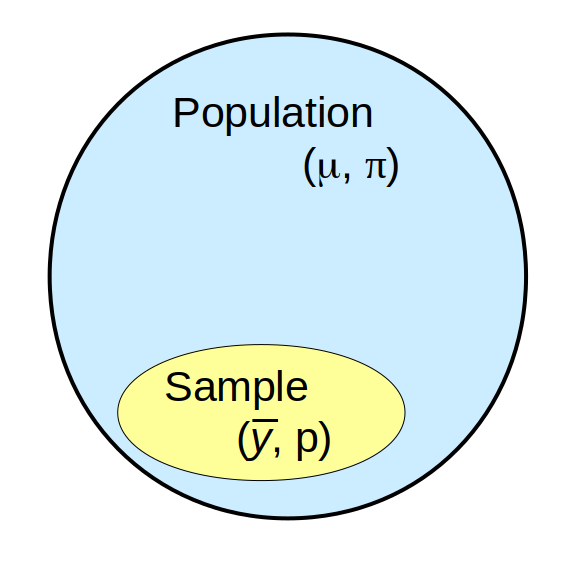
\includegraphics[scale=0.35]{../sampling_dist/MeansFig1.png}
}


\end{frame}




\begin{frame}[fragile]{Sampling Distributions}

\begin{knitrout}\scriptsize
\definecolor{shadecolor}{rgb}{0.969, 0.969, 0.969}\color{fgcolor}\begin{figure}

{\centering 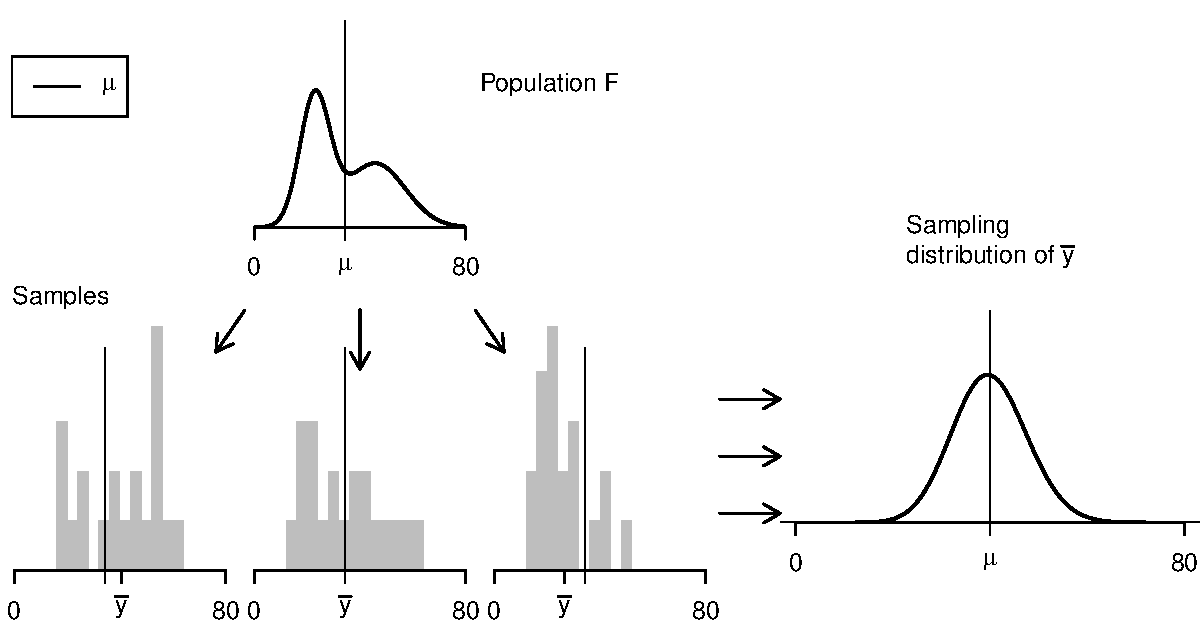
\includegraphics[width=1\linewidth]{figure/unnamed-chunk-1-1} 

}

\caption[Ideal world]{Ideal world. Sampling distributions are obtained by drawing repeated samples from the population, computing the statistic of interest for each, and collecting (an infinite number of) those statistics as the sampling distribution}\label{fig:unnamed-chunk-1}
\end{figure}


\end{knitrout}

\end{frame}


\begin{frame}[fragile]{Quadruple the work, half the benefit}

\framedgraphiccaption{../sampling_dist/ROOToceanAll.png}{When the sample size increases from 4 to 16, the spread of the sampling distribution for the mean is reduced by a half, i.e., the range is cut in half. This is known as the curse of the $\sqrt{n}$}
\end{frame}


\frame{\frametitle{The Central Limit Theorem (CLT)} 

\begin{itemize}
\item The sampling distribution of $\bar{y}$ is, for a large enough $n$, close to Gaussian in shape no matter what the shape of the distribution of individual $Y$ values. 
\item This phenomenon is referred to as the CENTRAL LIMIT THEOREM 
\item The CLT applied also to a \underline{sample proportion}, \underline{slope}, \underline{correlation}, or any other statistic created by \underline{aggregation of individual observations}
\end{itemize}

\begin{thm}[Central Limit Theorem]
\begin{center}
if $Y \sim ???(\mu_Y, \sigma_Y)$, then \\ \ \\
$\bar{y} \sim \mathcal{N}(\mu_Y, \sigma_Y / \sqrt{n})$
\end{center}
\end{thm}

\vspace{1.25cm}
%pause
}

\begin{frame}{Confidence Interval}

\begin{defm}[Confidence Interval]
A level $C$ confidence interval for a parameter has two parts:
\begin{enumerate}
\item An interval calculated from the data, \underline{usually} of the form $$\textrm{estimate} \pm \textrm{margin of error}$$ where the estimate is a sample statistic and the margin of error represents the accuracy of our guess for the parameter.
\item A confidence level $C$, which gives the probability that the interval will capture the true parameter value in \textit{different possible samples}. That is, the confidence level is the success rate for the method
\end{enumerate}
\end{defm}

%\framedgraphic{6899rule.png}

\end{frame}

\frame{\frametitle{Confidence Interval: A simulation study}

\vspace*{-0.1in}

\begin{figure}
\begin{center}
\epsfig{figure=../sampling_dist/Part3Figs/CIplots.eps,width=3.2in,height=2.7in}
\caption{\small{True parameter value is 2 (red line). Each horizontal black line represents a 95\% CI from a sample and contains the true parameter value. The blue CIs do not contain the true parameter value. 95\% of all samples give an interval that contains the population parameter.}}
\end{center}
\end{figure}
}


\begin{frame}{Interpreting a frequentist confidence interval}
\begin{itemize}
\setlength\itemsep{1em}
\item The confidence level is the success rate of the method that produces the interval.
\item We don't know whether the 95\% confidence interval from a \underline{particular
sample} is one of the 95\% that capture $\theta$ (the unknown population parameter), or one of the unlucky 5\% that miss. 
\item To say that we are \underline{95\% confident} that the unknown value of $\theta$
lies between $U$ and $L$ is shorthand for ``We got these numbers using a
method that gives correct results 95\% of the time.''
\end{itemize}
\end{frame}

\begin{frame}[fragile]{68\% Confidence interval using \texttt{qnorm}}




\vspace*{-0.09in}

\Wider[2em]{
\begin{knitrout}\scriptsize
\definecolor{shadecolor}{rgb}{0.969, 0.969, 0.969}\color{fgcolor}\begin{figure}

{\centering 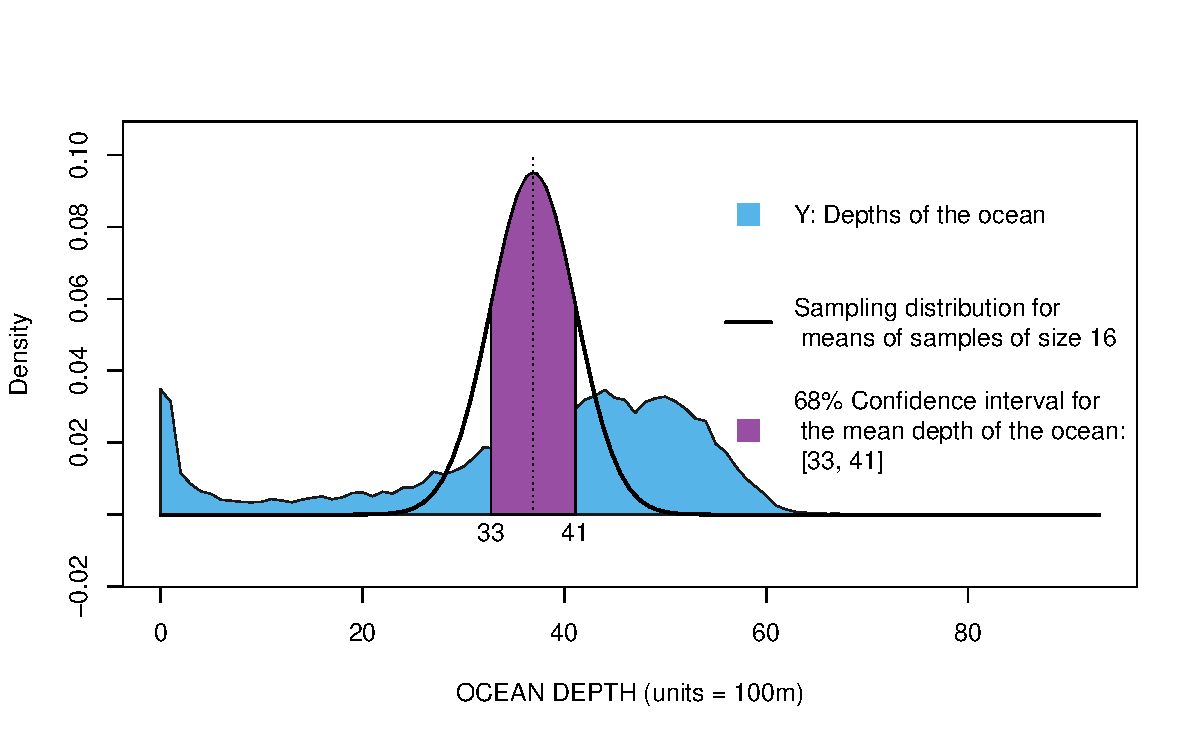
\includegraphics[width=1\linewidth]{figure/unnamed-chunk-3-1} 

}

\caption{68\% Confidence interval calculated using  \mbox{\texttt{qnorm(p = c(0.16,0.84), mean = 37, sd = 4.2)}}}\label{fig:unnamed-chunk-3}
\end{figure}


\end{knitrout}

}
\end{frame}



\begin{frame}[fragile]{95\% Confidence interval using \texttt{qnorm}}

\vspace*{-0.09in}


\Wider[2em]{
\begin{knitrout}\scriptsize
\definecolor{shadecolor}{rgb}{0.969, 0.969, 0.969}\color{fgcolor}\begin{figure}

{\centering 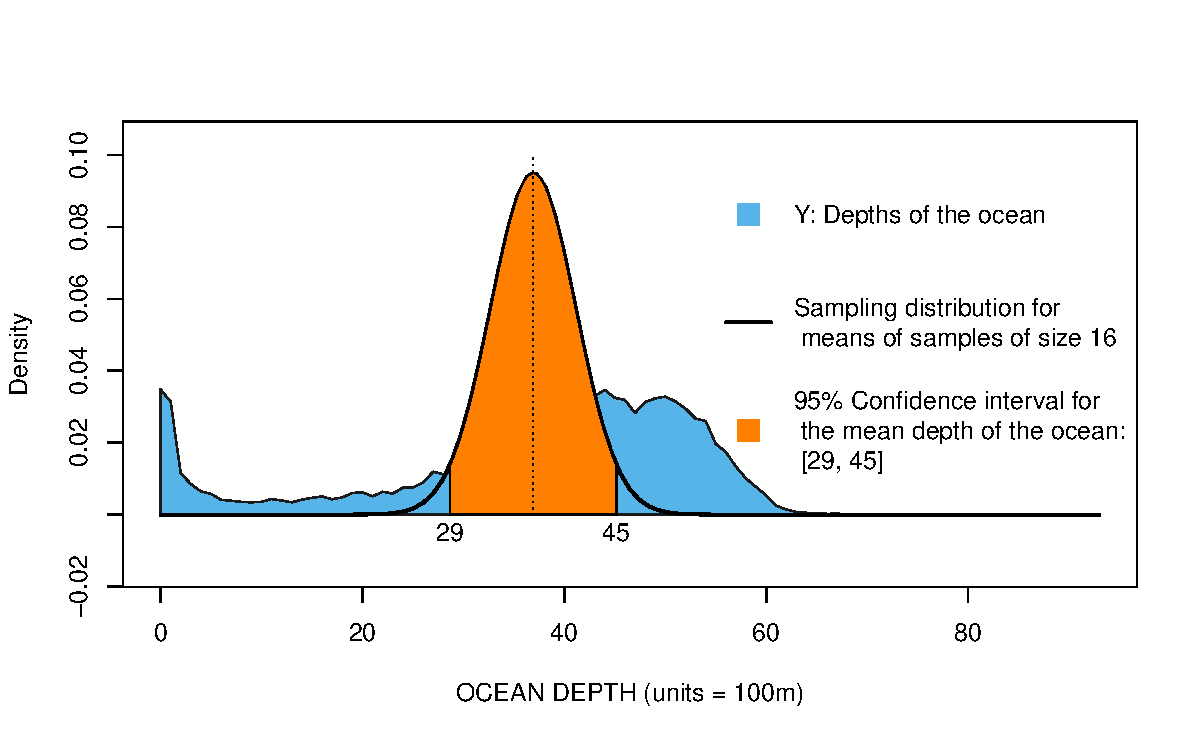
\includegraphics[width=1\linewidth]{figure/unnamed-chunk-4-1} 

}

\caption{95\% Confidence interval calculated using  \mbox{\texttt{qnorm(p = c(0.025,0.975), mean = 37, sd = 4.2)}}}\label{fig:unnamed-chunk-4}
\end{figure}


\end{knitrout}

}

\end{frame}

\frame{\frametitle{Example: Inference for a single population mean} So what
does the CI allow us to learn about $\mu$??
\begin{itemize}
\setlength\itemsep{2em}
\item It tells us that if we repeated this procedure again and again
(collecting a sample mean, and constructing a 95\% CI), 95\% of the
time, the CI would \textit{cover} $\mu$. 
\item That is, with 95\% probability, the \textit{procedure}
will include the true value of $\mu$. Note that we are making \underline{a probability statement about the CI}, not about the parameter. 
\item Unfortunately, \textcolor{blue}{we do not know whether the true value of $\mu$ is
contained in the CI in the particular experiment that we have
performed.}
\end{itemize}
}



\section{Bootstrap}

\begin{frame}{Motivation for the Bootstrap}
\begin{itemize}
	\setlength\itemsep{2em}
	\item The $\pm$ and \texttt{qnorm} methods to calculate a CI both require the CLT
\end{itemize}


\vspace*{0.2in}

\Large \textcolor{myblue}{Q: What happens if the CLT hasn't `kicked in`? Or you don't believe the CLT?} \\ \ \\

\pause 

\Large \textcolor{red}{A: Bootstrap} \\ \ \\
\end{frame}



\begin{frame}[fragile]{Reality: use the bootstrap distribution instead}




\framedgraphiccaption{../bootstrap/boot_diag.pdf}{\scriptsize{Bootstrap world. The bootstrap distribution is obtained by drawing repeated samples from an estimate of the population, computing the statistic of interest for each, and collecting those statistics. The distribution is centered at the observed statistic ($\bar{y}$), not the parameter ($\mu$).}}

\end{frame}


\begin{frame}[fragile]{Main idea: simulate your own sampling distribution}



\begin{knitrout}\scriptsize
\definecolor{shadecolor}{rgb}{0.969, 0.969, 0.969}\color{fgcolor}
\begin{alltt}
\hlkwd{library}\hlstd{(mosaic)}
\hlstd{s_dist} \hlkwb{<-} \hlkwd{do}\hlstd{(}\hlnum{10000}\hlstd{)} \hlopt{*} \hlkwd{mean}\hlstd{(} \hlopt{~} \hlstd{alt,} \hlkwc{data} \hlstd{=} \hlkwd{resample}\hlstd{(depths.n.20))}
\hlstd{CI_95} \hlkwb{<-} \hlkwd{quantile}\hlstd{(}\hlopt{~} \hlstd{mean,} \hlkwc{data} \hlstd{= s_dist,} \hlkwc{probs} \hlstd{=} \hlkwd{c}\hlstd{(}\hlnum{0.025}\hlstd{,} \hlnum{0.975}\hlstd{))}
\end{alltt}


{\centering 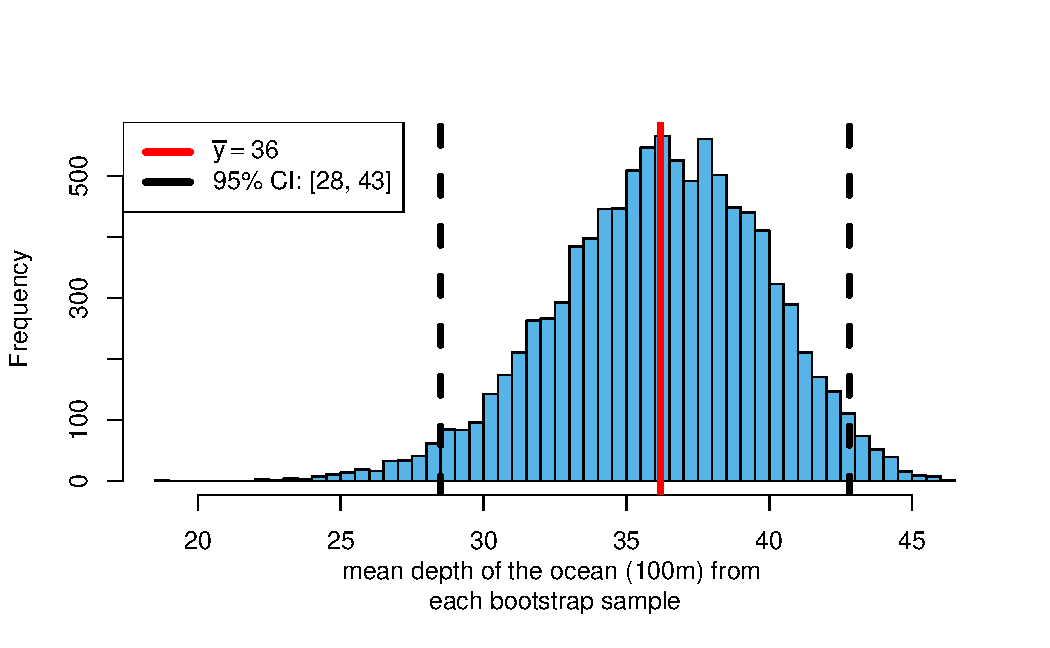
\includegraphics[width=1\linewidth]{figure/unnamed-chunk-7-1} 

}



\end{knitrout}

\end{frame}



\begin{frame}[fragile]{Example 1: Food intake and weight gain (A5-Q1)}

\begin{minipage}{0.47\textwidth}
\begin{knitrout}\scriptsize
\definecolor{shadecolor}{rgb}{0.969, 0.969, 0.969}\color{fgcolor}
\begin{tabular}{r|r|r|r}
\hline
subject & before & after & change\\
\hline
1 & 55.7 & 61.7 & 6.0\\
\hline
2 & 54.9 & 58.8 & 3.9\\
\hline
3 & 59.6 & 66.0 & 6.4\\
\hline
4 & 62.3 & 66.2 & 3.9\\
\hline
5 & 74.2 & 79.0 & 4.8\\
\hline
6 & 75.6 & 82.3 & 6.7\\
\hline
7 & 70.7 & 74.3 & 3.6\\
\hline
8 & 53.3 & 59.3 & 6.0\\
\hline
9 & 73.3 & 79.1 & 5.8\\
\hline
10 & 63.4 & 66.0 & 2.6\\
\hline
11 & 68.1 & 73.4 & 5.3\\
\hline
12 & 73.7 & 76.9 & 3.2\\
\hline
13 & 91.7 & 93.1 & 1.4\\
\hline
14 & 55.9 & 63.0 & 7.1\\
\hline
15 & 61.7 & 68.2 & 6.5\\
\hline
16 & 57.8 & 60.3 & 2.5\\
\hline
\end{tabular}


\end{knitrout}

\begin{knitrout}\tiny
\definecolor{shadecolor}{rgb}{0.969, 0.969, 0.969}\color{fgcolor}
\begin{alltt}
\hlkwd{mean}\hlstd{(weight}\hlopt{$}\hlstd{change)}
\end{alltt}
\begin{verbatim}
## [1] 4.73125
\end{verbatim}
\begin{alltt}
\hlkwd{sd}\hlstd{(weight}\hlopt{$}\hlstd{change)} \hlopt{/} \hlkwd{sqrt}\hlstd{(}\hlnum{16}\hlstd{)}
\end{alltt}
\begin{verbatim}
## [1] 0.4364362
\end{verbatim}

\end{knitrout}

\end{minipage}
\begin{minipage}{0.5\textwidth}
	\pause 
\begin{itemize}
	\small
	\setlength\itemsep{1em}
	\item 95\% CI for the mean weight change: 4.73 $\pm$ qt(p = c(0.025, 0.975), df = 16-1)$\times$ 0.44 
	\item $p$-value: pt(q = (4.73 - 0)/0.44, df=16-1, lower.tail=F)$\times$2 $<$ 0.001 
	\item This is a paired design $\to$ statistically valid to take difference and perform one-sample inference
	\item You can also bootstrap the \texttt{change}.
\end{itemize}
\end{minipage}

\end{frame}


\begin{frame}[fragile]{Example 1: Food intake and weight gain (A5-Q1) contd.}

\begin{minipage}{0.47\textwidth}




\begin{knitrout}\scriptsize
\definecolor{shadecolor}{rgb}{0.969, 0.969, 0.969}\color{fgcolor}
\begin{tabular}{r|r|r}
\hline
subject & Time & value\\
\hline
1 & 0 & 55.7\\
\hline
1 & 1 & 61.7\\
\hline
2 & 0 & 54.9\\
\hline
2 & 1 & 58.8\\
\hline
3 & 0 & 59.6\\
\hline
3 & 1 & 66.0\\
\hline
4 & 0 & 62.3\\
\hline
4 & 1 & 66.2\\
\hline
5 & 0 & 74.2\\
\hline
5 & 1 & 79.0\\
\hline
6 & 0 & 75.6\\
\hline
6 & 1 & 82.3\\
\hline
7 & 0 & 70.7\\
\hline
7 & 1 & 74.3\\
\hline
8 & 0 & 53.3\\
\hline
8 & 1 & 59.3\\
\hline
\end{tabular}


\end{knitrout}

\vspace*{1cm}

\small
Will a regression on this data provide the same results?

	
\end{minipage}
\begin{minipage}{0.5\textwidth}
	\pause 
	
\begin{knitrout}\tiny
\definecolor{shadecolor}{rgb}{0.969, 0.969, 0.969}\color{fgcolor}
\begin{verbatim}
Coefficients:
            Estimate Std. Error t value Pr(>|t|)
(Intercept)    65.74       2.51   26.20   <2e-16
Time            4.73       3.55    1.33     0.19

Residual standard error: 10 on 30 degrees of freedom
Multiple R-squared: 0.0559,	Adjusted R-squared: 0.0245 
F-statistic: 1.78 on 1 and 30 DF,  p-value: 0.192 
\end{verbatim}

\end{knitrout}

	\begin{itemize}
	\small
	\setlength\itemsep{2em}
	\item Point estimate is the same but standard error is much larger. Why? \pause 
	\item Hint: Think about assumptions for inference.
\end{itemize}

\end{minipage}

\end{frame}



\begin{frame}[fragile]{Ex. 2: Does breast-feeding weaken bones? (A4-Q3)}

\begin{minipage}{0.47\textwidth}
\begin{knitrout}\scriptsize
\definecolor{shadecolor}{rgb}{0.969, 0.969, 0.969}\color{fgcolor}
\begin{tabular}{l|l|r}
\hline
  & type & mineral\_loss\\
\hline
1 & Other & 2.4\\
\hline
5 & Other & 1.0\\
\hline
47 & Breast-feeding & -5.2\\
\hline
48 & Breast-feeding & -2.0\\
\hline
49 & Breast-feeding & -2.1\\
\hline
\end{tabular}



{\centering 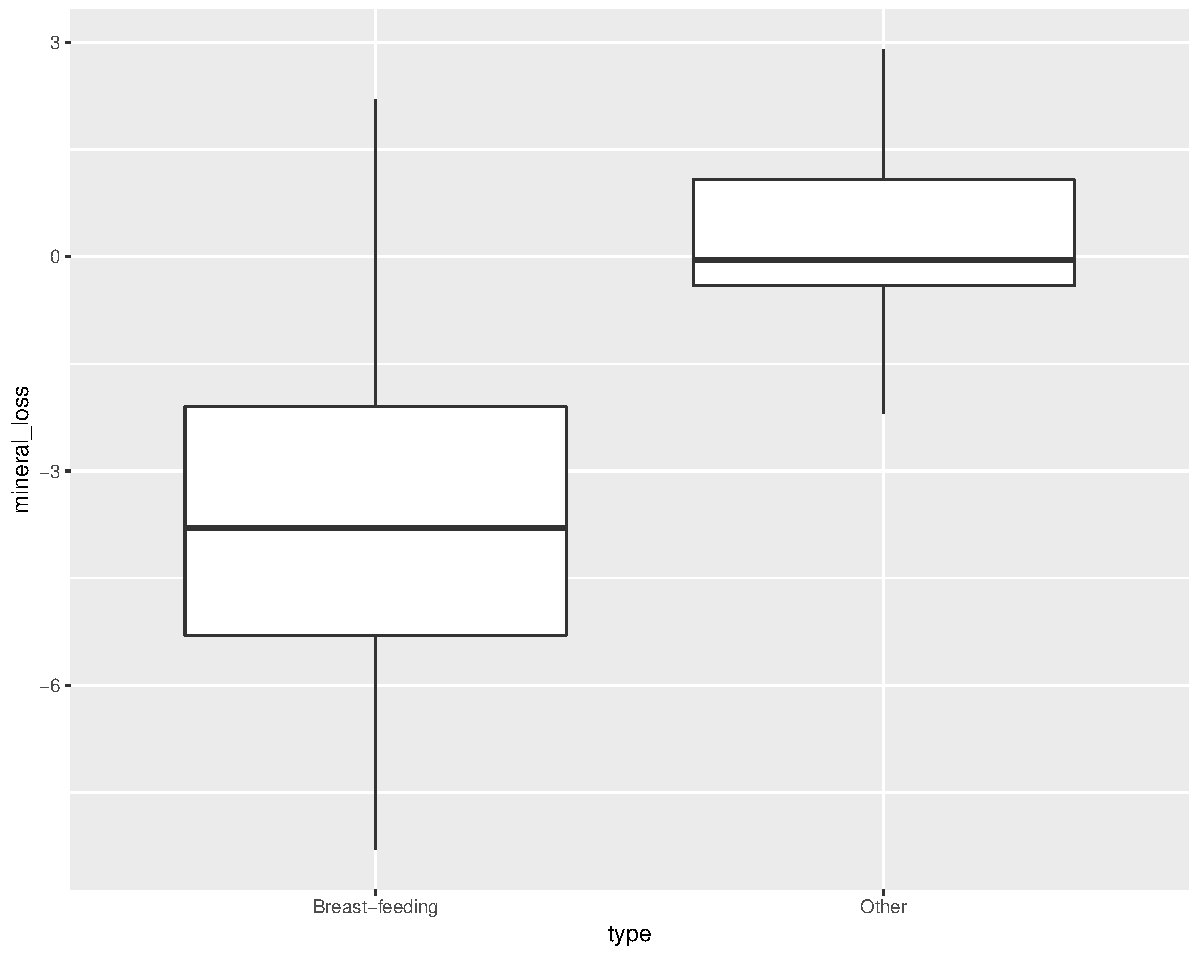
\includegraphics[width=1\linewidth]{figure/unnamed-chunk-13-1} 

}



\end{knitrout}
	
\end{minipage}
\begin{minipage}{0.5\textwidth}
	\pause 
	\begin{itemize}
		\small
		\setlength\itemsep{1em}
		\item  Researchers compared 47 breast-feeding women with 22 women of similar age who were neither pregnant nor lactating.
		\item Is this a paired design?
		\item How can we test if the data show distinctly greater bone mineral loss among the breast-feeding women?
	\end{itemize}
\end{minipage}

\end{frame}


\begin{frame}[fragile]{Ex. 2 contd. (A4-Q3)}
	\begin{itemize}
	\small
	\setlength\itemsep{1em}
	\item  We could run a linear regression (equivalently a two-sample t.test with equal variances):
\end{itemize}

\begin{knitrout}\tiny
\definecolor{shadecolor}{rgb}{0.969, 0.969, 0.969}\color{fgcolor}
\begin{verbatim}
## Call: lm(formula = mineral_loss ~ type, data = boneloss)
## 
## Coefficients:
##             Estimate Std. Error t value Pr(>|t|)
## (Intercept)   -3.587      0.321  -11.18  < 2e-16
## typeOther      3.896      0.568    6.86  2.7e-09
## 
## Residual standard error: 2.2 on 67 degrees of freedom
## Multiple R-squared: 0.412,	Adjusted R-squared: 0.404 
## F-statistic:   47 on 1 and 67 DF,  p-value: 2.73e-09
\end{verbatim}
\begin{alltt}
\hlcom{# remember that var.equal=FALSE is the default in t.test }
\hlkwd{t.test}\hlstd{(mineral_loss} \hlopt{~} \hlstd{type,} \hlkwc{data} \hlstd{= boneloss,} \hlkwc{var.equal} \hlstd{=} \hlnum{TRUE}\hlstd{)}
\end{alltt}
\begin{verbatim}
##  Two Sample t-test with mineral_loss by type 
## t = -6.8569, df = 67, p-value = 2.73e-09
## alternative hypothesis: true difference in means is not equal to 0 
## 95 percent confidence interval:
##  -5.030524 -2.762126 
## sample estimates:
## mean in group Breast-feeding          mean in group Other 
##                   -3.5872340                    0.3090909
\end{verbatim}

\end{knitrout}


\end{frame}



\begin{frame}[fragile]{Ex. 2 contd. (A4-Q3)}
\begin{itemize}
	\small
	\setlength\itemsep{1em}
	\item  Two-sample t.test with unequal variances
\end{itemize}

\begin{knitrout}\tiny
\definecolor{shadecolor}{rgb}{0.969, 0.969, 0.969}\color{fgcolor}
\begin{alltt}
\hlcom{# remember that var.equal=FALSE is the default in t.test }
\hlkwd{t.test}\hlstd{(mineral_loss} \hlopt{~} \hlstd{type,} \hlkwc{data} \hlstd{= boneloss)}
\end{alltt}
\begin{verbatim}
## Welch Two Sample t-test with mineral_loss by type 
## t = -8.4985, df = 66.197, p-value = 3.325e-12
## alternative hypothesis: true difference in means is not equal to 0 
## 95 percent confidence interval:
##  -4.811641 -2.981008 
## sample estimates:
## mean in group Breast-feeding          mean in group Other 
##                   -3.5872340                    0.3090909
\end{verbatim}

\end{knitrout}

\pause 
\begin{itemize}
	\small
	\setlength\itemsep{1em}
	\item  Or we could bootstrap (if we suspected CLT hasn't kicked in, or non-normal population distributions) each group separately and calculate the means. Then take the difference of these means as the sampling distribution for the difference in bone mineral loss. (See A4-Q3 Bonus)
\end{itemize}

\end{frame}





\section{One sample mean}


\begin{frame}{$\sigma$ known vs. unknown}
\begin{center}
	\begin{tabular}{|l|c|c|} \hline
		$\sigma$& known & unknown \\ \hline Data & $\{y_1,y_2,...,y_n\}$ &
		$\{y_1,y_2,...,y_n\}$\\
		& & \\
		Pop'n param & $\mu$ & $\mu$\\
		& & \\
		Estimator & $\overline{y} = \frac{1}{n}\sum_{i=1}^n y_i$ & $\overline{y} = \frac{1}{n}\sum_{i=1}^n y_i$ \\
		& & \\
		SD & $\sigma$ & $s = \sqrt{\frac{\sum_{i=1}^n(y_i-\overline{y})^2}{n-1}}$ \\
		& & \\
		SEM & $\sigma/\sqrt{n}$ & $s / \sqrt{n}$ \\
		& & \\
		$(1-\alpha)100$\% CI & $\overline{y} \pm z^\star_{1-\alpha/2}$(SEM) & $\overline{y} \pm t^\star_{1-\alpha/2, (n-1)}$(SEM) \\
		& & \\
		test statistic & $\frac{\overline{y}-\mu_0}{\textrm{SEM}}\sim \mathcal{N}(0,1)$ &
		$\frac{\overline{y}-\mu_0}{\textrm{SEM}}\sim t_{(n-1)}$ \\
		\hline
	\end{tabular}
\end{center}
\end{frame}


\begin{frame}{Assumptions}
\Wider[3em]{
\begin{center}
	\begin{tabular}{|l|c|c|c|} \hline
		& $z$ & $t$ & Bootstrap \\ 
		\hline 
		SRS & \cmark &\cmark &	\cmark\\
		& & & \\
		Normal population & \cmark$^\star$ & \cmark$^\star$ &  \xmark\\
		& & &\\
		needs CLT &  \cmark$^\star$ & \cmark$^\star$ &  \xmark\\
		& & &\\
		$\sigma$ known  & \cmark & \xmark & \xmark\\
		& & &\\
		Sampling dist. center at & $\mu$ & $\mu$ & $\bar{y}$\\
		& & &\\
		SD & $\sigma$ & $s$ & $s$ \\
		& & &\\
		SEM & $\sigma/\sqrt{n}$ & $s / \sqrt{n}$ & SD(bootstrap statistics) \\
		\hline
	\end{tabular}
	
	\footnotetext[1]{*If population is Normal then CLT is not needed. If population is not Normal then CLT is needed.}
\end{center}
}
\end{frame}



\begin{frame}{Means, Rates/Counts, Proportions}
\Wider[3em]{
				\scriptsize
	\begin{center}
		\begin{tabular}{|l|c|c|c|} \hline
			& mean & rate/count & proportion \\ 
			\hline 
			Parameter & $\mu$ & $\lambda$/$\mu$ ($\mu=\lambda\times PT$) &	$\pi$\\
			& & & \\
			Statistic & $\bar{y}$ & $\hat{\lambda}$/$y$ or $\hat{\mu}$ &  $p$ or $\hat{\pi}$\\
			& & &\\
			Distribution &  Normal($\mu$, $\sigma$), $t_{(df)}$ & Poisson($\mu$) &  Binomial(n, $\pi$)\\
			& & &\\
			CI for small $n$  & $\bar{y} \pm$ qt($\cdot$, df=n-1)$\times$SEM & qgamma($\cdot$,shape=c(y,y+1))$^c$ & Clopper-Pearson\\
			& & &\\
			CI for large$^d$ $n$  & qnorm($\cdot$, $\bar{y}$,SEM) & qnorm($\cdot$,$y$,$\sqrt{y}$) & qnorm($\cdot$, $p$, $\sqrt{\frac{p(1-p)}{n}}$)\\
			& & &\\
			$p$value small$^{a}$ $n$& pt & ppois & pbinom \\
			& & &\\
			$p$value large$^{a}$ $n$& pnorm & pnorm & pnorm \\
			\hline
		\end{tabular}
		
		\footnotetext[1]{need to specify lower.tail=FALSE}
				\footnotetext[2]{All inference requires SRS}
					\footnotetext[3]{qgamma gives CI for the count. Divide by PT if you want CI for the rate.}
			\footnotetext[4]{For Normal and Poisson $n>30$. For Binomial, $np > 10, n(1-p)>10$}
				
	\end{center}
}
\end{frame}



\section{One sample proportion}


\begin{frame}
\Wider[5em]{	
	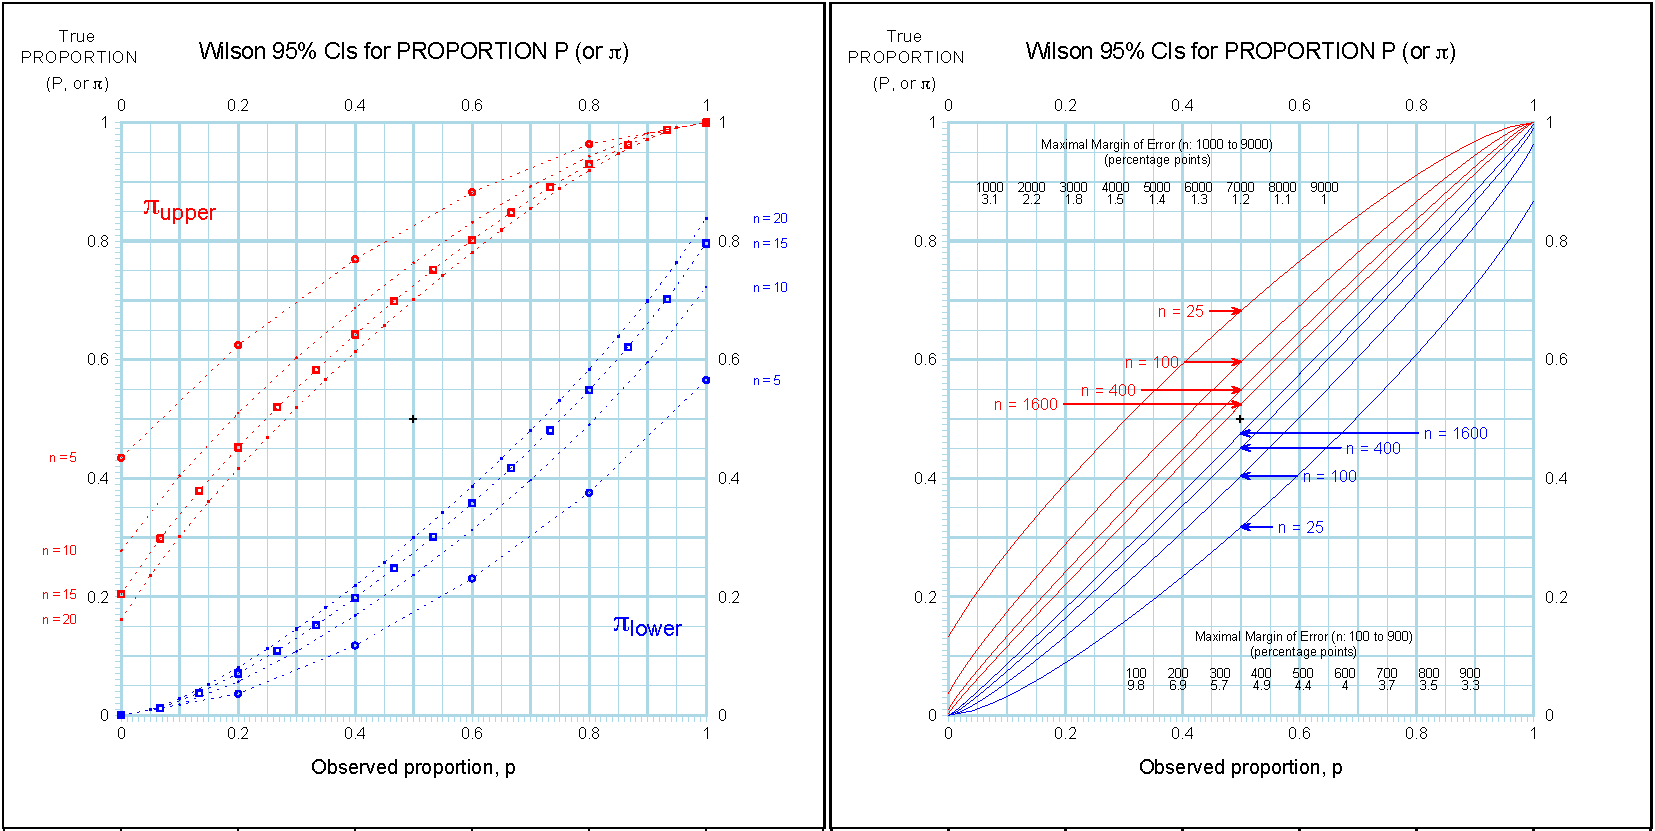
\includegraphics[width=4.95in,height=3.7in]{../one_sample_prop/Nomogram.pdf}
}
\end{frame}

\section{p-values}

\begin{frame}
\frametitle{$p$-values and statistical tests}


%\vspace{18pt}
\begin{defm}[$p$-value]
	A \textbf{probability concerning the observed data}, calculated under a \textbf{Null Hypothesis} assumption, i.e., assuming that the only factor operating is sampling or measurement variation. 
\end{defm}

\begin{itemize} 
	\item[\underline{Use}] To assess the evidence provided by the sample data
	in relation to a pre-specified claim or `hypothesis' concerning some parameter(s) or data-generating process. 
	\item[\underline{Basis}] As with a confidence interval, it makes use of the concept of a \textit{distribution}. 
	\item[\underline{Caution}] A $p$-value is NOT the probability that the null `hypothesis' is true
\end{itemize}
\end{frame}




\section{Regression}

\begin{frame}{Tidy data}

\begin{itemize}
	\setlength\itemsep{.51em}
	\item Each variable forms a column.
	\item Each observation forms a row.
	\item Each type of observational units forms a table
	\item Tidy data is ready for regression routines and plotting
\end{itemize}


\framedgraphic{tidy.png}

\end{frame}



\section{Varia}

\begin{frame}{Other remarks}

\begin{itemize}
	\setlength\itemsep{.51em}
	\item Statistical evidence $\to$ point estimate, confidence interval, $p$-value
\end{itemize}




\end{frame}


























\section{Examples}



\begin{frame}{Comparing two sun block lotions}

\begin{example}
	Your company produces a sun block lotion designed to protect the skin from both UVA and UVB exposure to the sun. You hire a company to compare your product with the product sold by your major competitor. The testing company exposes skin on the back of a sample of 20 people to UVA and UVB rays and measures the protection provided by each product. For 13 of the subjects, your product provided better protection. Do you have evidence to support a commercial claiming that your product provides superior UVA and UVB protection?
\end{example}


\end{frame}



\begin{frame}[fragile]{Comparing two sun block lotions}
\small
\begin{enumerate}
	\setlength\itemsep{1em}
	\item State the null hypothesis in words. \pause
	\item State the hypotheses in statistical notation \pause
	\begin{itemize}
			\setlength\itemsep{.71em}
		\item We need to first define the reference (null) distribution. Then the parameter of interest \pause
		\item Binomial(n=20, $\pi$=0.5) is the reference distribution where $\pi$ is the proportion of people who would receive superior UVA and UVB protection from your product. \pause
		The following are all equivalent: 
		\item[] $H_0: \pi = 0.5 \qquad$ $H_a: \pi > 0.5$ \pause
		\item[] $H_0: \pi_{\textrm{your product}}=\pi_{\textrm{their product}} = 0.5 \qquad$ $H_a: \pi_{\textrm{your product}} > \pi_{\textrm{their product}}$ \pause
		\item[] $H_0: \pi_{\textrm{your product}}-\pi_{\textrm{their product}} = 0 \qquad$ $H_a: \pi_{\textrm{your product}} > \pi_{\textrm{their product}}$ \pause
		\item You must define your own $\alpha$. Here we choose $\alpha=0.05$ 		
	\end{itemize}
      
 
\end{enumerate}

\end{frame}




\begin{frame}[fragile]{Comparing two sun block lotion - p-value}
\small
\begin{enumerate}
	\setlength\itemsep{.51em}
	
	\item Exact $p$-value:
\begin{knitrout}\scriptsize
\definecolor{shadecolor}{rgb}{0.969, 0.969, 0.969}\color{fgcolor}
\begin{alltt}
\hlkwd{pbinom}\hlstd{(}\hlnum{12}\hlstd{,} \hlnum{20}\hlstd{,} \hlnum{0.5}\hlstd{,} \hlkwc{lower.tail} \hlstd{=} \hlnum{FALSE}\hlstd{)}
\end{alltt}
\begin{verbatim}
## [1] 0.131588
\end{verbatim}
\begin{alltt}
\hlnum{1} \hlopt{-} \hlkwd{pbinom}\hlstd{(}\hlnum{12}\hlstd{,} \hlnum{20}\hlstd{,} \hlnum{0.5}\hlstd{)}
\end{alltt}
\begin{verbatim}
## [1] 0.131588
\end{verbatim}

\end{knitrout}
	\pause 

	\item Approximate $p$-value assuming Normal approximation is ok ($20 \times 0.5 \geq 10$ and $20 \times (1-0.5) \geq 10$)
\begin{knitrout}\scriptsize
\definecolor{shadecolor}{rgb}{0.969, 0.969, 0.969}\color{fgcolor}
\begin{alltt}
\hlstd{SEp} \hlkwb{<-} \hlkwd{sqrt}\hlstd{(}\hlnum{0.5}\hlopt{*}\hlnum{0.5}\hlopt{/}\hlnum{20}\hlstd{)} \hlcom{# under the null}
\hlstd{zstat} \hlkwb{<-} \hlstd{(}\hlnum{0.65} \hlopt{-} \hlnum{0.5}\hlstd{)} \hlopt{/} \hlstd{SEp}
\hlkwd{pnorm}\hlstd{(zstat,} \hlkwc{lower.tail} \hlstd{=} \hlnum{FALSE}\hlstd{)}
\end{alltt}
\begin{verbatim}
## [1] 0.08985625
\end{verbatim}

\end{knitrout}
	
	
	
\end{enumerate}

\end{frame}




\begin{frame}[fragile]{Comparing two sun block lotion - Exact 95\% CI}
\small
\begin{enumerate}
	\setlength\itemsep{1em}
	
	\item Exact CI (Clopper-Pearson or Nomogram):
\begin{knitrout}\scriptsize
\definecolor{shadecolor}{rgb}{0.969, 0.969, 0.969}\color{fgcolor}
\begin{alltt}
\hlstd{mosaic}\hlopt{::}\hlkwd{binom.test}\hlstd{(}\hlkwc{x} \hlstd{=} \hlnum{13}\hlstd{,} \hlkwc{n} \hlstd{=} \hlnum{20}\hlstd{,} \hlkwc{p} \hlstd{=} \hlnum{0.5}\hlstd{,}
\hlkwc{ci.method} \hlstd{=} \hlstr{"Clopper-Pearson"}\hlstd{,}
\hlkwc{alternative} \hlstd{=} \hlstr{"greater"}\hlstd{)}
\end{alltt}
\begin{verbatim}
 with 13 out of 20 
number of successes = 13, number of trials = 20, p-value = 0.1316
alternative hypothesis: true probability of success is greater than 0.5 
95 percent confidence interval:
 0.4419655 1.0000000 
sample estimates:
probability of success 
                  0.65 
\end{verbatim}

\end{knitrout}
	

	
\end{enumerate}

\end{frame}







\begin{frame}[fragile]{Comparing two sun block lotion - Approximate 95\% CI}
\small
\begin{enumerate}
	\setlength\itemsep{1em}
	
	\item Approximate 95\% CI:
\begin{knitrout}\scriptsize
\definecolor{shadecolor}{rgb}{0.969, 0.969, 0.969}\color{fgcolor}
\begin{alltt}
\hlstd{mosaic}\hlopt{::}\hlkwd{binom.test}\hlstd{(}\hlkwc{x} \hlstd{=} \hlnum{13}\hlstd{,} \hlkwc{n} \hlstd{=} \hlnum{20}\hlstd{,} \hlkwc{p} \hlstd{=} \hlnum{0.5}\hlstd{,}
\hlkwc{ci.method} \hlstd{=} \hlstr{"Wald"}\hlstd{,}
\hlkwc{alternative} \hlstd{=} \hlstr{"greater"}\hlstd{)}
\end{alltt}
\begin{verbatim}
Exact binomial test (with Wald CI) with 13 out of 20 
number of successes = 13, number of trials = 20, p-value = 0.1316
alternative hypothesis: true probability of success is greater than 0.5 
95 percent confidence interval:
 0.4745704 1.0000000 
sample estimates:
probability of success 
                  0.65 
\end{verbatim}

\end{knitrout}
	
		
	\item Approximate 95\% CI assuming Normal approximation is ok 
\begin{knitrout}\scriptsize
\definecolor{shadecolor}{rgb}{0.969, 0.969, 0.969}\color{fgcolor}
\begin{alltt}
\hlkwd{qnorm}\hlstd{(}\hlkwd{c}\hlstd{(}\hlnum{0.025}\hlstd{,} \hlnum{0.975}\hlstd{),} \hlkwc{mean} \hlstd{=} \hlnum{0.65}\hlstd{,} \hlkwc{sd} \hlstd{=} \hlkwd{sqrt}\hlstd{(}\hlnum{0.65}\hlopt{*}\hlnum{0.35} \hlopt{/} \hlnum{20}\hlstd{))}
\end{alltt}
\begin{verbatim}
## [1] 0.4409627 0.8590373
\end{verbatim}

\end{knitrout}
	
\end{enumerate}

\end{frame}




\end{document}
